\subsection{nonlinear quantization}	
\begin{frame}\frametitle{sampling and quantization}\framesubtitle{SNR and PDF}
		\begin{equation}
			SNR = 6.02\cdot w + c_{\mathrm{S}}\quad [dB]
		\end{equation}
		\pause
        \bigskip
		$\Rightarrow c_{\mathrm{S}}$ depends on signal's PDF (and scaling)
		\begin{table}
			\centering
			\begin{footnotesize}
				\begin{tabular}{clc}
				\hline
				\textbf{PDF} & \textbf{SNR}\\
				\hline
				square wave & $c_S =  10.80$\\
				sine wave & $c_S =  1.76$\\
				rect & $c_S =  0$\\
				tri & $c_S \approx  -3$\\
				Gauss & $c_S \approx  -7$\\
				Laplace & $c_S \approx  -9$\\
				speech & $c_S \approx  -10\ldots -15$\\
				\hline
				\end{tabular}
			\end{footnotesize}
		\end{table}
	\end{frame}	
	\begin{frame}\frametitle{sampling and quantization}\framesubtitle{SNR and PDF modification}
		idea: quantize frequent signal values at higher resolution:
		
		\pause
		\begin{itemize}
			\item \textbf{approach 1 }	
				\begin{enumerate}
					\item	flatten PDF (companding)
					\item	linear quantization
					\item	extract signal (expanding)
				\end{enumerate}
			\pause
            \only<2>{
            \begin{figure}
                \begin{center}
                    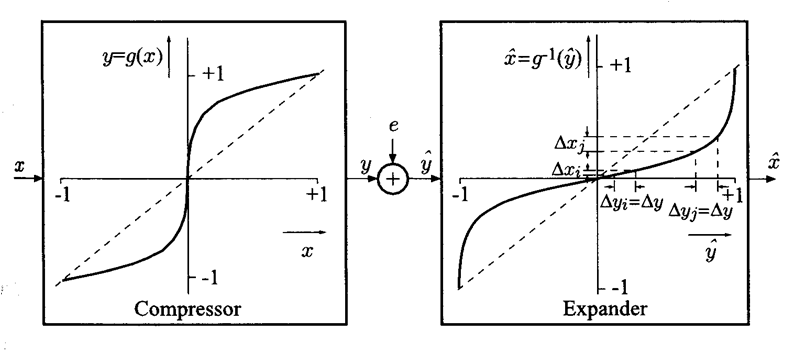
\includegraphics[scale=0.5]{Graph/quant_compexp}
                \end{center}
            \end{figure}
            }
            \pause
            \item \textbf{approach 2 }	
				\begin{enumerate}
					\item	adapt quantization step size to PDF
				\end{enumerate}

		\end{itemize}
	\end{frame}	

	\begin{frame}\frametitle{sampling and quantization}\framesubtitle{A Law quantization 1/3}
		\begin{equation}
			F(x)	= sign(x)\left\lbrace
					\begin{array}{ll} 
			          \frac{A|x|}{1+\log(A)}, & |x| \leq \frac{1}{A}\\ 
			          \frac{1+\log(A|x|)}{1+\log(A)}, & \frac{1}{A} \leq |x| \leq 1\\ 
          			\end{array} 
          			\right.
		\end{equation}
		\begin{equation}
			F^{-1}(y)	= sign(y)\left\lbrace
					\begin{array}{ll} 
			          \frac{|y|(1+\log(A))}{A}, & |y| \leq \frac{1}{1+\log(A)}\\ 
			          \frac{\exp\big(|y|(1+\log(A))-1\big)}{A}, & \frac{1}{1+\log(A)} \leq |y| \leq 1\\ 
          			\end{array} 
          			\right.
		\end{equation}
		$A = 87.7$
	\end{frame}	

	\begin{frame}\frametitle{sampling and quantization}\framesubtitle{A Law quantization 2/3}
	    \begin{figure}
			\centering
				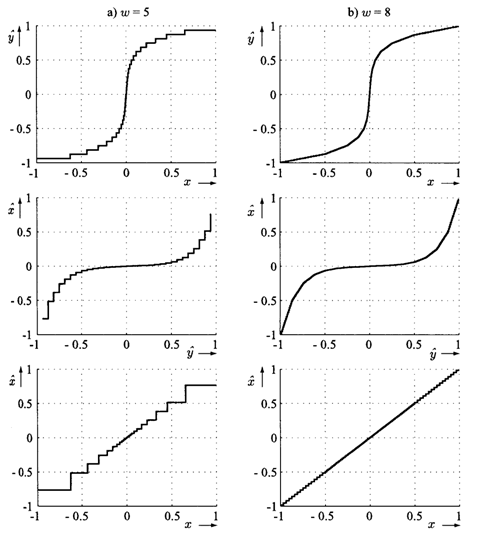
\includegraphics[scale=0.5]{Graph/a-law}
		\end{figure}
	\end{frame}

	\begin{frame}\frametitle{sampling and quantization}\framesubtitle{A Law quantization 2/3}
	    \vspace{-5mm}
        \begin{figure}
			\centering
				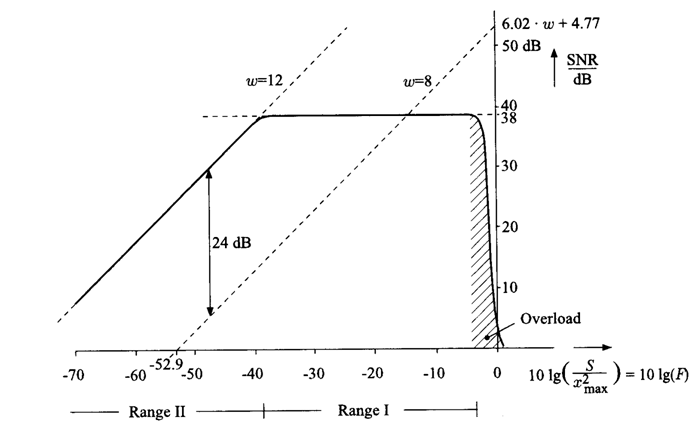
\includegraphics[scale=0.5]{Graph/snr_a-law}
		\end{figure}
        \begin{itemize}
            \item   range 1: linear
            \item   range 2: log
        \end{itemize}
	\end{frame}
